\newpage
\section{Progettazione}
Si è scelto di utilizzare XHTML 1.0 strict e CSS 3.0 per garantire una buona compatibilità con i browser non aggiornati, in modo tale da non ostacolare gli utenti con dispositivi più datati.
Il gruppo ha deciso di adottare la strategia \textit{Responsive Web} per coniugare le esigenze di diversi dispositivi. L'utilizzo di CSS 3.0 è stato indispensabile per l'impiego delle flexbox per la configurazione della struttura a faccette della pagina contenente la lista dei prodotti.

\subsection{Struttura organizzativa} 
Si è scelto di utilizzare la struttura gerarchica perché è alla base di una buona architettura di sistema e perché risulta essere familiare all'utente, garantendo il facile sviluppo di uno modello mentale. Il sito è basato su una gerarchia ampia e poco profonda (viene utilizzata una gerarchia ampia di profondità massima 2 livelli).
Nella pagina che visualizza l'intera lista dei prodotti abbiamo adottato una struttura a faccette poiché risulta essere familiare agli utenti, in quanto convenzione esterna dettata dal mercato dei siti di E-Commerce più affermati.

\subsection{Mobile first}
Non si è adottata la strategia \textit{Mobile First} perché è stata consigliata a lezione dopo l'inizio dello sviluppo del sito. Le pagine realizzate non sono ricche di elementi superflui per cui è risultato semplice riordinare i contenuti. Sono state invece riscontrate più difficoltà per l'ordinamento del header, per quanto riguarda il posizionamento dei pulsanti \textbf{Accedi} e \textbf{Carrello}.

\subsection{Above the fold}
Il contenuto del sito è minimale e limitato ai soli elementi essenziali, pertanto tutti i contenuti informativi fondamentali, il logo e gli strumenti di navigazione sono raggiungibili senza effettuare scroll eccessivo (lo scroll è presente nelle pagine che ne richiedono un impiego indispensabile per il corretto ridimensionamento del contenuto come nel caso della pagina che visualizza la lista dei prodotti acquistabili).

\subsection{Responsive Web}
Per implementare il \textit{responsive web} sono stati definiti 3 intervalli, secondo i seguenti punti di rottura:
\begin{itemize}
    \item \textbf{Mobile (280px - 767px)}: si è scelto di non definire un ulteriore punto di rottura nel mezzo poiché  il layout degradava in modo elegante, per cui si è deciso di non implementare ulteriori fogli di stile;
    \item \textbf{Desktop grandi (768px - 1200px)}: questo intervallo è stato fondamentale per fornire un corretto ridimensionamento di header e footer, che sviluppandosi orizzontalmente (senza questo intervallo) non fornivano una degradazione elegante. In particolare il foglio di stile associato a tale intervallo è associato alla visualizzazione del sito nei computer portatili;
    \item \textbf{Desktop molto grandi (min 1201px)}: questo intervallo è quello in cui è stato sviluppato il sito in prima battuta. 
\end{itemize}

\subsection{Database}
A supporto del comportamento è stato creato un database relazionale, allo scopo di tenere traccia di prodotti, utenti e transazioni. Il database è in 2NF:
\begin{itemize}
    \item è in 1NF;
    \item tutti gli attributi non chiave dipendono dall'intera chiave.
\end{itemize}
\begin{figure}[H]
\centering
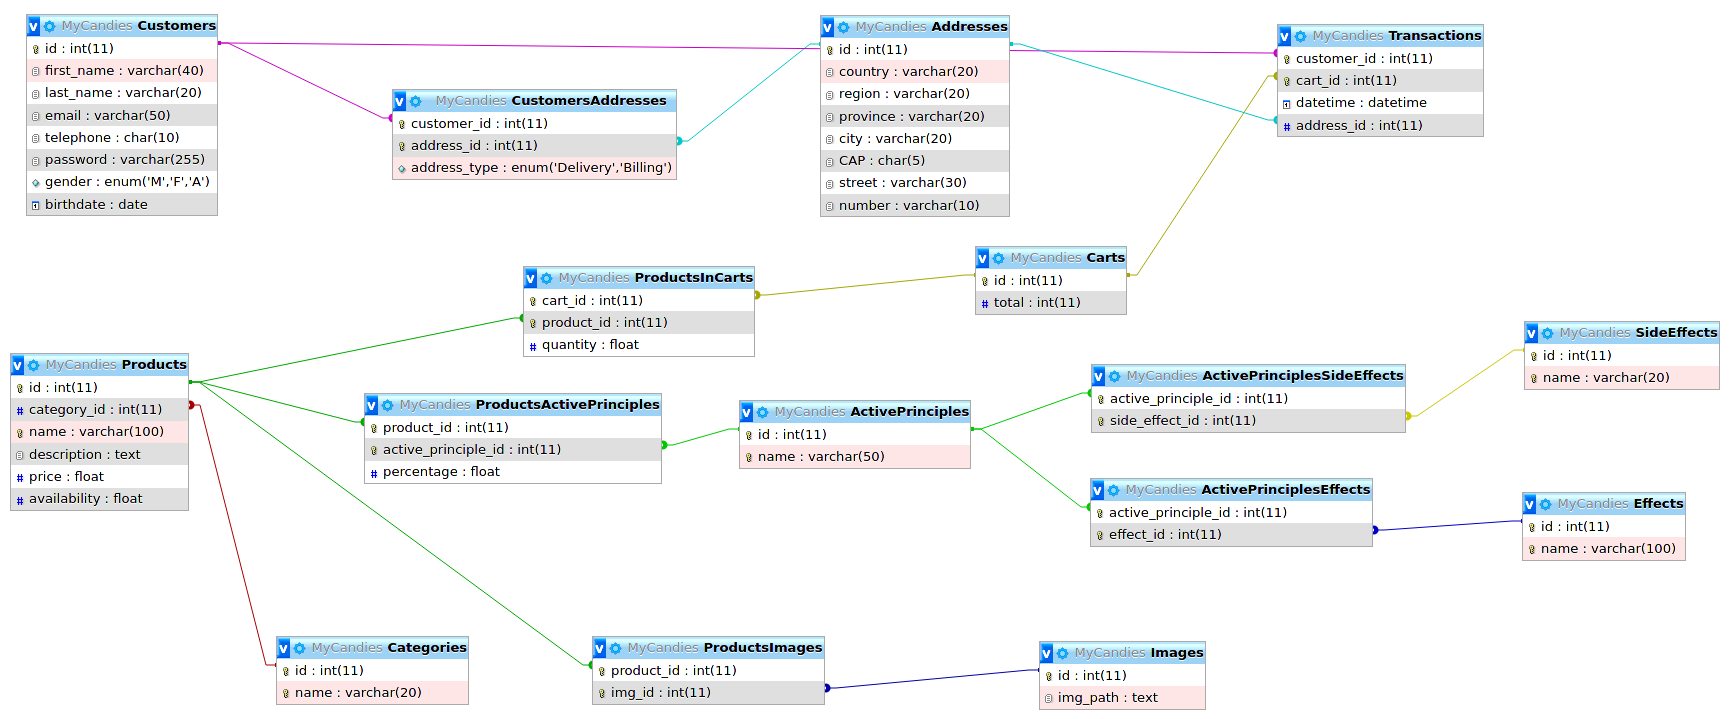
\includegraphics[width=\textwidth]{modello_relazionale}
\caption{Modello relazionale del database di My Candies} 
\end{figure}

\subsubsection{Products} Ad ogni prodotto è collegata una categoria, uno o più principi attivi, effetti ed effetti collaterali:  \begin{itemize}
    \item[] \textbf{ActivePrinciples}: è possibile che un prodotto abbia più principi attivi, in quanto la relazione tra Products e ActivePrinciples è molti a molti. Tuttavia non è stata prevista nella vista la possibilità di collegare più principi attivi ad una solo prodotto;
    \item[] \textbf{Effects e SideEffects}: queste entità contengono effetti ed effetti collaterali dei principi attivi, ogni principio attivo può avere 0 o più effetti ed effetti collaterali.
    \item[] \textbf{Images}: questa entità contiene i path delle immagini utilizzate per i prodotti. La relazione tra i prodotti e le immagini è molti a molti, è quindi possibile avere più immagini per un solo prodotto, questa caratteristica non è però utilizzabile dall'interfaccia grafica;
    \item[] \textbf{Categories}: ogni prodotto è identificato da una categoria.
\end{itemize}
\subsubsection{Customers} Ogni cliente è identificato da un id. È possibile per un cliente avere più indirizzi:
 \begin{itemize}
    \item[] \textbf{Addresses}: l'entità Addresses contiene gli indirizzi degli utenti ed è in relazione molti a molti con l'entità Customers, è quindi possibile avere più indirizzi per un solo utente, questa caratteristica non è disponibile nell'interfaccia, ogni utente può avere un solo indirizzo.
\end{itemize}
\subsubsection{Gestione delle transazioni} Tramite le entità ProductsInCarts, Carts, Transactions sono gestiti carrello e transazioni:
\begin{itemize}
    \item[] \textbf{Carts}: rappresenta il carrello, ogni carrello è identificato da un id;
     \item[] \textbf{ProductsInCarts}: è il risultato della relazione molti a molti tra Products e Carts, in questo modo è possibile avere lo stesso prodotto in più carrelli e più prodotti in un carrello;
    \item[] \textbf{Transactions}: rappresenta l'acquisto da parte del cliente, una transazione è identificata dal cliente e dal carrello.
\end{itemize}
Diverse caratteristiche del database non sono state poi implementate nell'interfaccia grafica. La base dati è quindi scalabile e reattiva ad eventuali aggiornamenti di My Candies.

\subsection{Accessibilità}
Per garantire l'accessibilità si è cercato di attenersi alle linea guida viste nel corso di \textit{Tecnologie Web}. Per avere un risconto quanto più preciso per attestare l'accessibilità del sito si è seguito lo standard europeo WCAG 2.0.
\subsubsection{Separazione tra presentazione, struttura e comportamento}
Ognuna di queste 3 componenti è stata realizzata mantenendo una completa separazione. 
La \textit{struttura} è stata realizzata con XHTML per garantire il supporto anche ai più vecchi browser ancora in circolazione ed evitando l'utilizzo di tag deprecati, garantendo così l'assenza di discriminazione tecnologica.
Non si sono utilizzati tag html a fini presentazionali, come l'utlizzo delle tabelle per l'ordinamento del layout.
La parte di \textit{presentazione} è stata realizzata tramite l'applicazione di fogli di stile importati. Per garantire la separazione non sono state definite applicazione di stile inline o embedded.
La parte di \textit{comportamento} realizzata tramite Javascript assicura una degradazione elegante. Javascript è stato utilizzato solamente per il controllo dei form lato client e per la visualizzazione mobile. Nei mobile dato il poco spazio a disposizione si è scelto di implementare un menù a comparsa. Nel caso in cui Javascript non funzionasse o fosse disattivato non verrebbe effettutata alcuna modifica, lasciando il menù visibile e privo di tasto per aprire/chiudere il menù. Quindi nel caso di problemi il menù sarebbe sempre accessibile ed utilizzabile.
\subsubsection{Aiuti alla navigazione}
 L'accessibilità è stata garantita anche attraverso altri strumenti utili all'orientamento e alla navigazione.
 \begin{itemize}
     \item \textbf{Breadcrumb}: le breadcrumb rappresentato la lista di pagine visitate per arrivare alla pagina corrente, che è l'unica senza link. E' utile all'utente perché permette di capire dove si trova, come è arrivato in una data pagina e come poter eventualmente tornare alle pagine precedenti. Ogni breadcrumb comincia con il testo "Ti trovi in:" per esplicitare il ruolo di quest'ultima;
     \item \textbf{Link}: sono stati inseriti diversi link per facilitare la navigazione. In fondo ad ogni pagina, prima del footer, è presente un link "Torna su" per tornare rapidamente al header. Alcuni di questi con la medesima funzione sono nascosti nelle versioni desktop per renderli visibili agli screen reader. 
     I link nascosti sopra citati sono resi disponibili a tutti gli utenti nella versione mobile, per garantire un rapido ritorno senza effettuare molto scroll.
     Nel header sono presenti, a seconda delle pagine, dei link visibili agli screen reader per passare al contenuto della pagina, saltando le voci di menù che risulterebbero ripetitive.
     \item \textbf{Marcatori HTML}: Per rendere il sito accessibile si è fatto un corretto uso dei marcatori.
     Le tabelle solo state utilizzate solamente per la rappresentazione ordinata dei dati. Sapendo che gli screen reader linearizzano le tabelle sono stati utilizzati tutti i tag utili a renderle accessibili (summary, scope, etc..). Sono stati esplicitati i linguaggi naturali utilizzando l'attributo "lang" per indicare parole in lingua diversa da quella italiana. Si è fatto uso del tag "abbr" ove necessario. Queste accortezze servono a garantire una corretta lettura del testo da parte degli screen reader.
 \end{itemize}